\documentclass[twoside]{article}

\usepackage[math]{kurier}
\usepackage[sc]{mathpazo}
\renewcommand{\sfdefault}{kurier}

\usepackage[boxruled]{algorithm2e}
\usepackage[utf8]{inputenc}
\usepackage[backend=biber]{biblatex}
\usepackage[english]{babel}
\usepackage[english]{babel}
\usepackage[autostyle]{csquotes}
\usepackage{placeins}
\usepackage[backend=biber]{biblatex}
\bibliography{./lecture_11_biblio_.bib}
\usepackage{hyperref}
\usepackage{graphics}
\usepackage{graphicx}
\usepackage{subcaption}
\usepackage{amsmath}
\usepackage{float}
\setlength{\oddsidemargin}{0.25 in}
\setlength{\evensidemargin}{-0.25 in}
\setlength{\topmargin}{-0.6 in}
\setlength{\textwidth}{6.5 in}
\setlength{\textheight}{8.5 in}
\setlength{\headsep}{0.75 in}
\setlength{\parindent}{0 in}
\setlength{\parskip}{0.1 in}


\newcounter{lecnum}
\renewcommand{\thepage}{\thelecnum-\arabic{page}}
\renewcommand{\thesection}{\thelecnum.\arabic{section}}
\renewcommand{\theequation}{\thelecnum.\arabic{equation}}
\renewcommand{\thefigure}{\thelecnum.\arabic{figure}}
\renewcommand{\thetable}{\thelecnum.\arabic{table}}


\newcommand{\lecture}[3]{
   \pagestyle{myheadings}
   \thispagestyle{plain}
   \newpage
   \setcounter{lecnum}{#1}
   \setcounter{page}{1}
   \noindent
   \begin{center}
   \framebox{
      \vbox{\vspace{2mm}
    \hbox to 6.28in { {\bf \sffamily AA 274: Principles of Robotic Autonomy
                        \hfill Winter 2018} }
       \vspace{4mm}
       \hbox to 6.28in { {\sffamily{\Large \hfill Lecture #1: #2  \hfill}} }
       \vspace{2mm}
       % \hbox to 6.28in { {\it \hfill Scribes: #4} }
      \vspace{2mm}}
      
   }
   \end{center}
   \markboth{Lecture #1: #2}{Lecture #1: #2}

   \vspace*{4mm}
}


%%%%%%%%%%%%%%%%%%%%%%%%%%
%document
\begin{document}
%modify this
\lecture{12}{Markov Localization and EKF-localization}{}

\section{Introduction}
The aim of these notes is to help you learn about Markov localization with an emphasis on Extended Kalman Filter (EKF) localization. The algorithms covered in these notes will begin to solve the problem of determining the current pose of the robot based on a map of the environment and data from the robot's sensors. These probabilistic map-based localization techniques address realistic issues of noise and uncertainty in robotic data and often out-perform alternative techniques when applied to the real world.\\
\\
These lecture notes will cover the following topics:
\begin{itemize}
    \item Casting the localization problem within a Bayesian Filtering Framework
    \item Maps
    \item Markov Localization
    \item Extended Kalman Filter (EKF) Localization
    \item A Taxonomy of Localization Problems
\end{itemize}

\section{Casting the localization problem within a Bayesian Filtering Framework}

\subsection{Terminology}
As in the general filtering context, at time t, the state is given by $x_t$
, the control input is given by $u_t$ , and the measurements are given by the observation $z_t$. For a differential drive robot equipped with a laser range-finder (returning a set of range $r_i$ and bearing $\phi_i$ measurements), we have

\begin{equation}
x _ { t } = \left( \begin{array} { l } { x } \\ { y } \\ { \theta } \end{array} \right) \quad u _ { t } = \left( \begin{array} { c } { v } \\ { \omega } \end{array} \right) \quad z _ { t } = \left\{ \left( \begin{array} { c } { r _ { i } } \\ { \phi _ { i } } \end{array} \right) \right\} _ { i }
\end{equation}


\subsection{Strategy and Ingredients of probabilistic map-based localization}

The general strategy for the robot localization problem occurs in two steps: First, during the prediction (or
action) update, the robot estimates its position through proprioception (such as encoders or dead reckoning)
The uncertainty of the robot during this phase increases due to the accumulation of odometric error
(through integrating over time). The second step is the perception (or measurement, or correction) update,
where the robot uses exteroceptive sensors (such as ultrasonic, laser, camera) to correct its earlier estimated
prediction. The uncertainty of the robot configuration shrinks. By combining these two steps, a robot can
localize with respect to its map.
In order to solve the robot localization problem, the following ingredients are needed:

\begin{itemize}
    \item Initial probability distribution, $bel(x0)$ for the initial robot location.
    \item Map of the environment. If not known \emph{a priori}, then it can be built.
    \item Data from robotic sensors including the observation $z_t$ and the control input $u_t$
    \item Probabilistic motion model. Derived from robotic kinematics, the current location, x, is a function of previous location, $x_t$, and control input $u_t$, with additional modeled error distributions.
    \item Probabilistic measurement model. This model is derived from the sensor measurements of the robot. It consists of the measurement function h depends on the environment map and the robot location and an added noise term such that the probability distribution peaks at the noise-free value.
\end{itemize}

\subsection{Maps}
A key ingredient to instantiate Bayes filtering in the context of localization is a map. A map m is a list of
objects in the environment along with their properties, given by

\begin{equation}
m = \left\{ m _ { 1 } , m _ { 2 } , \ldots , m _ { N } \right\}
\end{equation}

Each $m_i$
is an object that encapsulates some property of the environment. The two types of maps we will
focus on here are location-based maps and feature-based maps. As will be discussed further in the next
sections, different map types typically have a trade-off in computational efficiency and explicitness.

\subsubsection{Location-based maps}

For location-based maps, an index i corresponds to a specific location (and hence, they are volumetric).
Figure \ref{fig:LocationBasedMaps} shows two examples of location-based maps.

\begin{figure}[H]
\centering
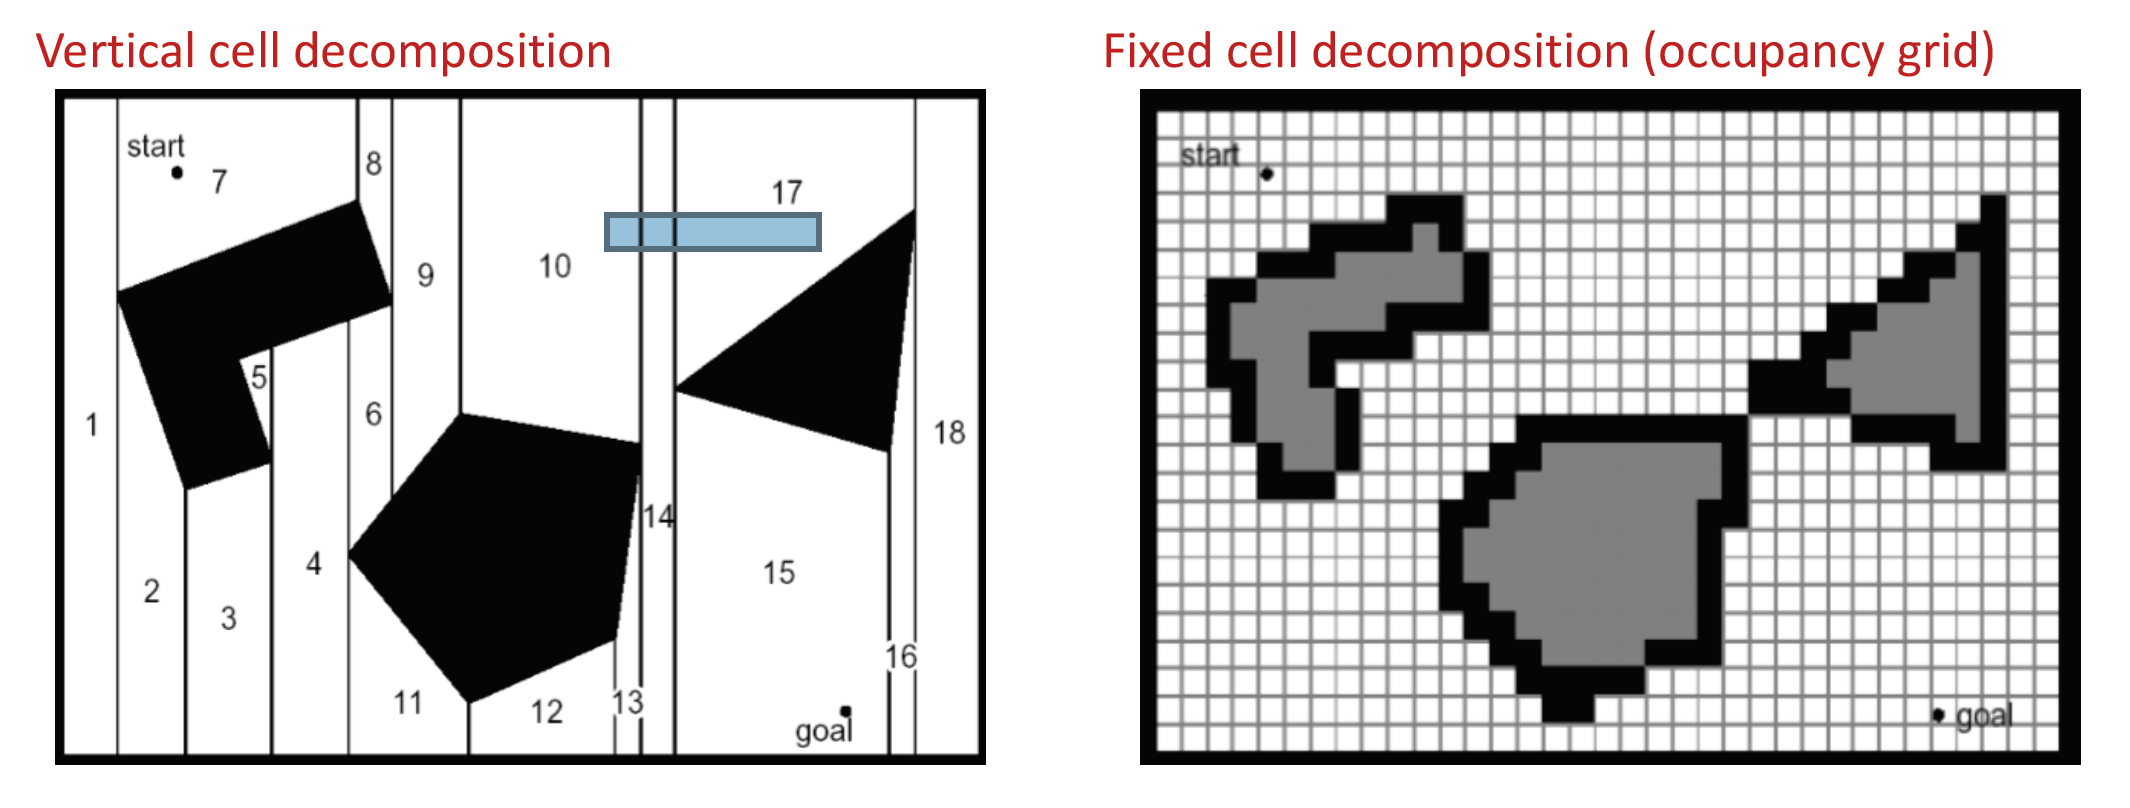
\includegraphics[width=.9\linewidth]{LBM.png}
\caption{Two examples of location-based maps.}
\label{fig:LocationBasedMaps}
\end{figure}

The first example of a location-based map employs vertical cell decomposition. This method essentially sweeps a vertical line through the width of the environment, and every time a corner is encountered, a cell is built. The result is a set of trapezoidal cells as shown in Fig. \ref{fig:LocationBasedMaps}, left. Each element of the map vector would be one of the cells. It is important to note that this technique can only describe the location of the robot using the presence or absence of the robot in a cell, but cannot give information on where within a cell the robot may be. The second common example of a location-based map uses fixed cell decomposition (Fig. \ref{fig:LocationBasedMaps}, right). In this grid map, the $i$th element of the map corresponds to the vector $x_i$ position of the i-th cell of the grid map. Thus, each cell represents a map vector. As compared the the fixed cell decomposition, the vertical cell decomposition is more efficient, as it abstracts the environment as a graph with nodes and edges. However, fixed cell decomposition can have better spatial resolution at the expense of additional computational complexity. Both techniques can give both the presence and absence of an object, which cannot be done with feature-based maps.

\subsubsection{Feature-based maps}
For feature-based maps, an index i is a feature index, and mi contains, next to the properties of a feature, the Cartesian location of that feature. One can think of this type of map as a collection of landmarks, such as points or lines. Figure \ref{fig:FeatureBasedMaps} gives two examples of feature-based maps.

\begin{figure}[H]
\centering
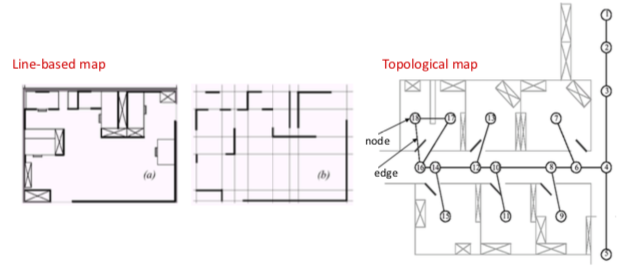
\includegraphics[width=.9\linewidth]{FeatureBasedMaps.png}
\caption{Two examples of feature-based maps.}
\label{fig:FeatureBasedMaps}
\end{figure}

The first example, the lined-based map, uses a line representation of the environment and is commonly
used in structured environments like buildings. This is the type of map that we will focus on in this class,
but the concepts covered on filtering and localization apply to all maps.
The second example is the topological map, which, rather than directly measuring geometric environmental
quantities, abstracts the environment as a collection of high level features. These features could be the
position of a chair or a lamp, for example.
These types of abstractions can improve the computational efficiency but feature-based maps cannot give
information on the presence and absence of a specific object in the environment.

\subsection{State Transition}
As we have seen previously, the motion model is probabilistic:
$p(x_t|u_t, x_t-1)$ describes the posterior distribution over the kinematic
states that the robot assumes when executing control $u_t$ when starting
from $x_t-1$. An illustration of this concept is shown in Figure \ref{fig:ProbabilisticMotion}. However, unlike what we have seen previously, we introduce
the map, which plays a role in the forward propagation of the dynamics.
It is important to note that $p(x_t|u_t, x_t-1) \neq p(x_t|u_t, x_t-1, m)$.
To understand why, consider the possible future states of the robot when it is next to a wall. If we do not consider the map, the model may erroneously give a non zero probability that the robot can travel through the obstacle.

\begin{figure}[H]
\centering
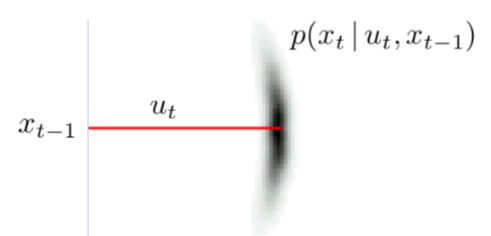
\includegraphics[width=.5\linewidth]{ProbabilisticMotion.png}
\caption{Probabilistic Motion}
\label{fig:ProbabilisticMotion}
\end{figure}

To avoid sampling from the state transition function, which is hard to do, a common technique is to make the approximation:

\begin{equation}
p \left( x _ { t } | u _ { t } , x _ { t - 1 } , m \right) \approx \eta \frac { p \left( x _ { t } | u _ { t } , x _ { t - 1 } \right) p \left( x _ { t } | m \right) } { p \left( x _ { t } \right) }
\end{equation}

The derivation of this approximation is as follows. Using Bayes theorem,

\begin{equation}
    p \left( x _ { t } | x _ { t - 1 } , u _ { t } , m \right) = \frac { p ( m | x _ { t } , x _ { t - 1 } , u _ { t } ) p \left( x _ { t } | x _ { t - 1 } , u _ { t } \right) } { p ( m | x _ { t - 1 } , u _ { t } ) }
\end{equation}

Because $p(m|x_{t-1}, u_t)$ is independent of $x_t$ we can include it in a normalizer, $\eta ^ \prime$, so

\begin{equation}
p \left( x _ { t } | x _ { t - 1 } , u _ { t } , m \right) = \eta ^ { \prime } p ( m | x _ { t } , x _ { t - 1 } , u _ { t } ) p \left( x _ { t } | x _ { t - 1 } , u _ { t } \right)
\end{equation}

Now we make the approximation that $p(m|x_t, x_{t-1}, u_t) \approx p(m|x_t)$, which neglects where we are coming from (discarding the information that says along a given motion, we might have an obstacle).

\begin{equation}
    p \left( x _ { t } | x _ { t - 1 } , u _ { t } , m \right) = \eta ^ { \prime } p ( m | x _ { t } ) p \left( x _ { t } | x _ { t - 1 } , u _ { t } \right)
\end{equation}

The last step involves using Bayes rule again to write $p(m|x_t) = p(x_t|m)p(m)/p(x_t)$. Because $p(m)$ is independent of $x_t$, we can include it in a normalizer: $\eta = \eta^{\prime} p(m)$.

Finally,

\begin{equation}
    p \left( x _ { t } | u _ { t } , x _ { t - 1 } , m \right) \approx \eta \frac { p \left( x _ { t } | u _ { t } , x _ { t - 1 } \right) p \left( x _ { t } | m \right) } { p \left( x _ { t } \right) }
    \label{pnormalized}
\end{equation}

$\eta$, the normalizing factor, is equal to one divided by the sum of the total probability of the rest of expression so that the resulting probability density function sums to 1. In general, the prior with respect to $x_t$ is uniform so the denominator in the final expression also gets included as a constant in the normalizer. Then, the terms that remain are the two probability functions in the numerator. The first is the probability distribution of the future state of the robot as if there were no obstacles. The second is the probability of x given m, which is essentially a consistency check that gives the plausibility of a state $x_t$ given a map. For example, in a grid world representation, the result could be a binary random variable, where the probability that the robot is in the same cell as an obstacle is 0 and otherwise the result is 1. This approximation essentially computes the state transition assuming no obstacles and then applies a consistency check. Next, we ground the measurement model in the map. The measurement model is probabilistic $p(z_t|x_t, m)$ and we have to condition with respect to a map because the observation also depends on the map. Sensors usually generate more than one measurement when queried, so we have batches of measurements $z_t = \{z_t^1, ..., z_t^K\}$ . This is the main difference with respect to the Bayes filter (where we were considering sequential measurements). Typically, for simplicity, we assume that these measurements are independent so that

\begin{equation}
    p \left( z _ { t } | x _ { t } , m \right) = \prod _ { k = 1 } ^ { K } p \left( z _ { t } ^ { k } | x _ { t } , m \right)
\end{equation}

\section{Markov Localization}

Markov localization uses a specified probability distribution across all possible robot positions. This high level instantiation of the Bayes filter in the context of localization is fairly straightforward as follows.

\begin{figure}[H]
\centering
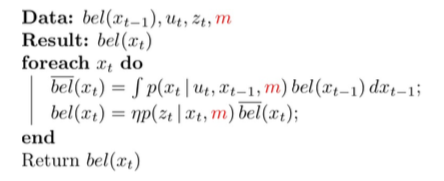
\includegraphics[width=.5\linewidth]{MarkovLocalizationAlgo.png}
\caption{Markov Localization Algorithm}
\label{fig:MarkovLocalizationAlgo}
\end{figure}

We input our belief pose at $t - 1$ given by $bel(x_{t-1})$, our control $u_t$, our measurement $z_t$, and the conditioning over the map $m$. The Markov localization model is conceptually identical to the Bayes filter except for the inclusion of $m$. 

Markov localization has the goal of iteratively propagating forward the belief over the pose of the robot in two steps. The first step is a prediction step that leverages the knowledge of the state transition function of the robot to go from $bel(x_{t-1})$ to $bel(x_t)$. The second step is the correction step that accounts for the measurement feedback. Figure 12.3 illustrates an example of this algorithm.

As is the case for Bayes filters, we must initialize the Markov localization algorithm with an initial belief $bel(x_0)$. For position tracking, if the initial pose is known,\\
\begin{equation}
    \operatorname { bel } \left( x _ { 0 } \right) = \left\{ \begin{array} { l l } { 1 } & { \text { if } x _ { 0 } = \overline { x } _ { 0 } } \\ { 0 } & { \text { otherwise } } \end{array} \right.
\end{equation}
If the initial pose is partially known,
\begin{equation}
    \operatorname { bel } \left( x _ { 0 } \right) \sim \mathcal { N } \left( \overline { x } _ { 0 } , \Sigma _ { 0 } \right)
\end{equation}
For global localization, where the initial pose is unknown, the belief is initialized as a uniform distribution
\begin{equation}
    b e l \left( x _ { 0 } \right) = 1 / | X |
\end{equation}
To make the Markov localization algorithm tractable, we need to add some structure to the representation of $bel(x_t)$. We can consider three representations. The next section will cover a Gaussian representation in
the context of EKF localization. Grid representations and particle filter representations will be covered in the next lecture.
\begin{figure}[H]
\centering
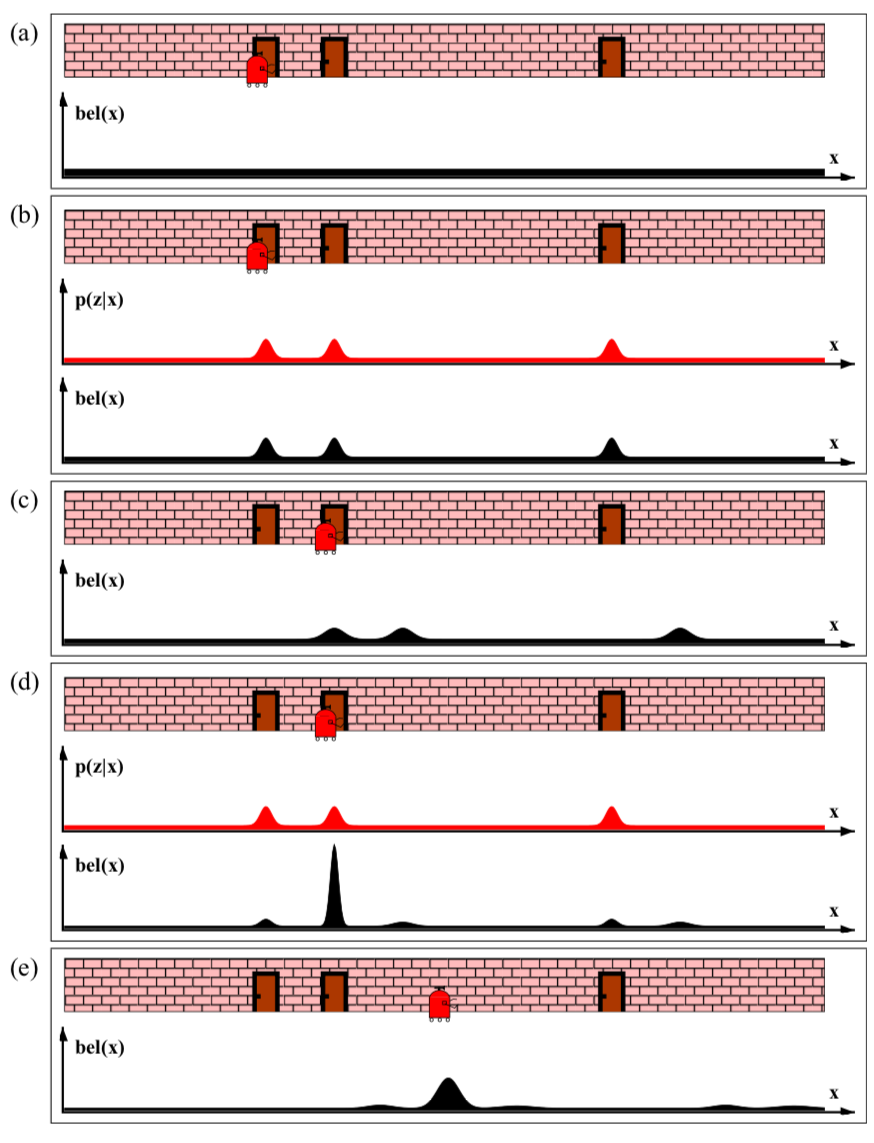
\includegraphics[width=.8\linewidth]{MarkovLocalizationPic.png}
\caption{Markov Localization Illustration. We consider a robot moving along a wall with three doors (a) The belief is initialized with a uniform distribution. (b) The robot moves to the first door and makes an observation. We apply the correction step to update our belief (c) The robot moves to the second door. The shifted belief is flattened because there is uncertainty with how much we moved. (d) We take a second observation, apply the correction, and obtain a large peak in the posterior belief. (e) The robot’s belief after moving further down the wall}
\label{fig:MarkovLocalizationPic}
\end{figure}

\section{Extended Kalman Filter (EKF) Localization}
The key idea of EKF localization is to represent the belief $bel(x_t)$ by its first and second moment, $\mu_t$ and
$\sum_t$. We will assume that a feature-based map is available, consisting of point landmarks, given by
\begin{align}
    m = \{m_1, m_2, \hdots\} \quad m_j = (m_{j,x}, m_{j,y})
\end{align}
where each $m_j$ encapsulates the location of the landmark in the global coordinate frame. We also assume
that we have a sensor that can measure the range $r$ and the bearing $\phi$ of the landmarks relative to the
robot’s local coordinate frame.

The range and bearing sensors measure a set of independent features at time $t$
\begin{align}
    z_t = \{z_t^1, z_t^2, \hdots \} = \{(r_t^1,\phi_t^1),(r_t^2,\phi_t^2), \hdots )
\end{align}
where each measurement $z_t^i$ contains the range $r_t^i$ and bearing $\phi_t^i$. We also instantiate a motion model
assuming a differential drive robot with states $(x, y, \theta)$.

Now that we’ve made assumptions about the map, measurements, and the robot motion, we can instantiate the measurement model which will allow us to re-derive the equations for the Markov localization filter. The measurement model tells us the likelihood of a given measurement given our state. Therefore, assuming that the $i$-th measurement at time $t$ corresponds to the $j$-th landmark in the map $m$, the measurement model is

\begin{align}
\left( \begin{array} { c } { r _ { t } ^ { i } } \\ { \phi _ { t } ^ { i } } \end{array} \right) = h \left( x _ { t } , j , m \right) + \mathcal { N } \left( 0 , Q _ { t } \right)
\end{align}
where $\mathcal{N}(0,Q_t)$ is the model's Gaussian noise and
\begin{equation}
    h \left( x _ { t } , j , m \right) = \left( \begin{array} { c } { \sqrt { \left( m _ { j , x } - x \right) ^ { 2 } + \left( m _ { j , y } - y \right) ^ { 2 } } } \\ { \operatorname { atan } 2 \left( m _ { j , y } - y , m _ { j , x } - x \right) - \theta } \end{array} \right)
    \label{hxjm}
\end{equation}
\subsection{Data Association}
The data association problem is the potential uncertainty about the identity of a landmark. For instance,
we may be given a range and bearing, but these measurements are not very meaningful if we do now
know what landmark they are given with respect to. As a result, for a map with $N$ total landmarks, we
define a \textit{correspondence variable} $c_t^i \in 1, ..., N + 1$ that relates measurement $z_t^i$ and landmark $m_j$, where
\begin{itemize}
    \item $c_t^i = j \leq N$ if the $i$-th measurement at time $t$ corresponds to the $j$-th landmark
    \item $c_t^i = N + 1$ if a measurement does not correspond to any landmark
\end{itemize}
There are two versions of the localization problem - when the correspondence variables are known, and
when they are not known. We generally only deal with the second case in practice, but to gain insight, we
start by discussing the first version.

\subsection{EKF Localization with Known Correspondences}
The EKF localization algorithm is derived from the EKF filter, but with two main differences - measurements are now associated with landmarks, and multiple measurements are processed at the same time. We begin again with our differential drive robot and assumption of the stochastic motion model (with some process disturbance $\epsilon$ that has a Gaussian distribution) and Jacobian $G$:
\begin{equation}
    x _ { t } = g \left( u _ { t } , x _ { t - 1 } \right) + \epsilon _ { t } , \quad \epsilon \sim \mathcal { N } \left( 0 , R _ { t } \right) , \quad G _ { t } : = J _ { g } \left( \mu _ { t } , \mu _ { t - 1 } \right)
\end{equation}
The (nonlinear) range and bearing measurement model $h(x_i, j, m)$ now includes the index j of the landmark with respect to which we are taking the measurements:
\begin{equation}
    z _ { t } ^ { i } = h \left( x _ { i } , j , m \right) + \delta _ { t } , \quad \delta _ { t } \sim \mathcal { N } \left( 0 , Q _ { t } \right) , \quad H _ { t } ^ { i } : = \frac { \partial h \left( \overline { \mu } _ { t , j , m } \right) } { \partial x _ { t } }
\end{equation}
Here $\delta$ is again the measurement noise, and $H$ is the measurement Jacobian. From differentiating \ref{hxjm},

\begin{figure}[H]
\centering
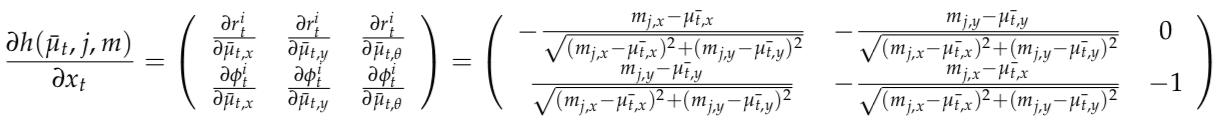
\includegraphics[width=.7\linewidth]{BigEquation.png}
\label{fig:BigPartialEquation}
\end{figure}

\begin{equation}
    Q _ { t } = \left( \begin{array} { c c } { \sigma _ { r } ^ { 2 } } & { 0 } \\ { 0 } & { \sigma _ { \phi } ^ { 2 } } \end{array} \right)
\end{equation}
The EKF localization algorithm is shown below. The key differences from the Bayes/EKF filter are the new
inputs (the correspondence variables ct and map m), and the fact that we are now considering batches of
measurements. As with the Bayes filter, we start with the prediction step, in which the mean and variance
are propagated using Taylor series expansions. We then carry out the correction step by exploiting the
conditional independence assumption for our batch of measurements,
\begin{equation}
    p \left( z _ { t } | x _ { t } , c _ { t } , m \right) = \prod _ { i } p \left( z _ { t } ^ { i } | x _ { t } , c _ { t } ^ { i } , m \right)
\end{equation}
which allows us to incrementally add information (i.e. process the measurements sequentially) as if there
was no motion between measurements.
\begin{figure}[H]
\centering
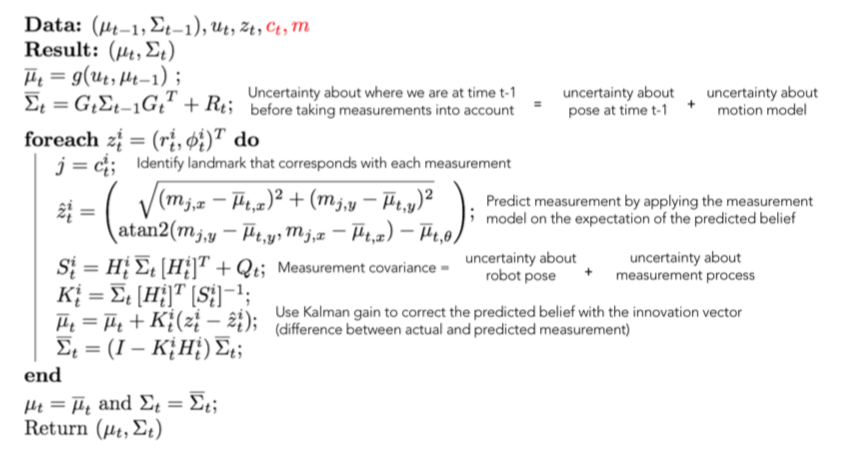
\includegraphics[width=.7\linewidth]{EKFLocalization.png}
\caption{EKF Localization with Known Correspondences}
\label{fig:EKFLocalization}
\end{figure}
The EKF-localization steps are illustrated for a differential drive robot in the following figures:
\begin{figure}[H]
\centering
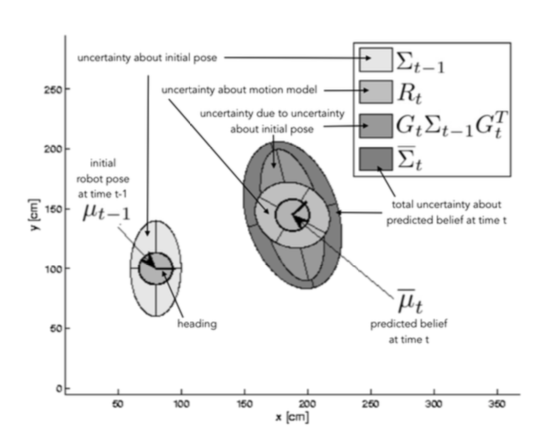
\includegraphics[width=.7\linewidth]{PredictionStep.png}
\caption{The prediction step. Observations measure the relative distance (range) and heading (bearing) of the robot to a landmark. We assume here that the robot detects only one landmark at a time.}
\label{fig:PredictionStep}
\end{figure}

\begin{figure}[H]
\centering
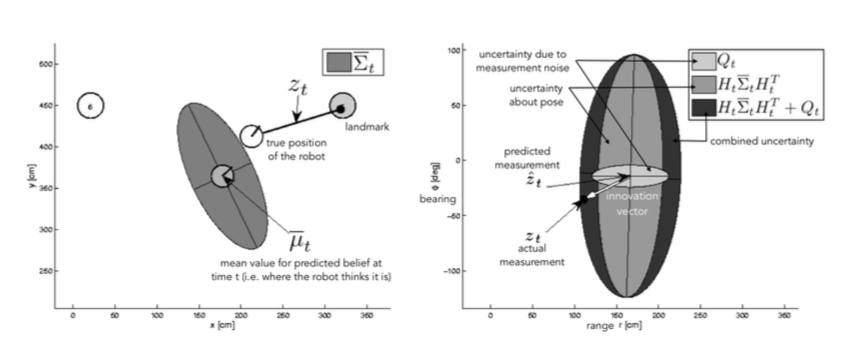
\includegraphics[width=.7\linewidth]{MeasurementPredictionStep.png}
\caption{The measurement prediction step. In this example, the measured range is much shorter than what was expected based on the predicted belief. The innovation vector, represented by the white arrow in the diagram on the right, shows the difference between the actual and predicted measurements.}
\label{fig:MeasurementStep}
\end{figure}

\begin{figure}[H]
\centering
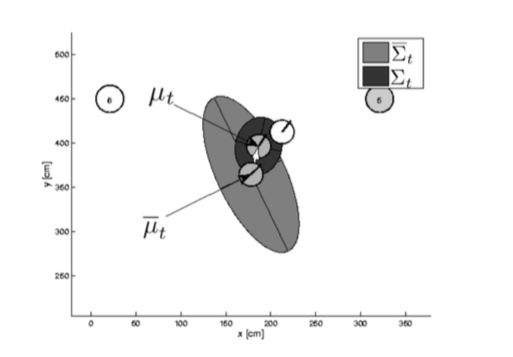
\includegraphics[width=.7\linewidth]{CorrectionStep.png}
\caption{The correction step. The expectation is corrected by moving in the direction indicated by the white innovation vector, resulting in an updated position that is closer to the true position (indicated by the white circle).}
\label{fig:MeasurementStep}
\end{figure}

\subsection{EKF Localization with Unknown Correspondences}
For EKF localization with unknown correspondences, we must jointly estimate the correspondence variables and use these estimates to implement the Markov filter. The simplest way to determine the identity of a landmark during localization is to use maximum likelihood estimation, in which the most likely value of the correspondences $c_t$ is determined by maximizing the data likelihood:
\begin{equation}
    \hat { c } _ { t } = \arg \max _ { c _ { t } } p \left( z _ { t } | c _ { 1 : t } , m , z _ { 1 : t - 1 } , u _ { 1 : t } \right)
\end{equation}
In other words, we pick the set of correspondence variables that maximizes the probability of getting the
measurement that we see, given the history of correspondence variables, the map, the history of measurements, and the history of controls. The value of $c_t$ is then taken for granted, so this method can be quite brittle; any mistake made during this process will propagate into the future.

The challenge with this method is that each element can take on many values (equal to the number of landmarks), and the number of possible combinations is exponential. The optimization problem is therefore
over an exponentially large physical space for a nonlinear function. As a result, we must resort to applying reasonable approximations with a model of independent measurements, and perform maximization
separately for each $z_t^i$.
\subsection{Estimating the Correspondence Variable}
The first step to solving the set of correspondence variables is to optimize the correspondence variables one by one:
\begin{equation}
    p \left( z _ { t } ^ { i } | c _ { 1 : t } , m , z _ { 1 : t - 1 } , u _ { 1 : t } \right)
\end{equation}
Essentially, we want to find the likelihood of $z_t^i$ given the conditions at c, m, z, and u. In order to do so, we use the total probability theorem. Through this method, we are optimizing the likelihood of each individual event instead of a joint optimization of all likelihood events at once. After algebraic manipulation, this translates to performing the following calculation:
\begin{equation}
p \left( z _ { t } ^ { i } | c _ { 1 : t } , m , z _ { 1 : t - 1 } , u _ { 1 : t } \right) \approx N \left( h \left( \overline { \mu } _ { t } , c _ { t } ^ { i } , m \right) , H _ { t } ^ { i } \overline { \Sigma } _ { t } \left[ H _ { t } ^ { i } \right] ^ { T } + Q _ { t } \right)
\end{equation}
What we get is that the probability of $z_t^i$ is approximately equal to the Gaussian distribution with mean equal to the predicted measurement. The next step is to find the correspondences using this Gaussian distribution with the following estimation:
\begin{equation}
\hat { c } _ { t } ^ { i } = \operatorname { argmax } p \left( z _ { t } ^ { i } | c _ { 1 : t } , m , z _ { 1 : t - 1 } , u _ { 1 : t } \right) \approx \operatorname { argmax } N \left( z _ { t } ^ { i } ; h \left( \overline { \mu } _ { t } , c _ { t } ^ { i } , m \right) , H _ { t } \overline { \Sigma } _ { t } H _ { t } ^ { T } + Q _ { t } \right)
\end{equation}

Very similar to the EKF with known correspondences, we apply an algorithm very similar to the one for EKF localization for known parameters. This includes a maximum likelihood estimator for the correspondence variables, and we are now no longer assuming the correspondence variables are inputs but rather optimizing for their values.The general outline of the algorithm is to do prediction, estimation, correspondences between measurements and landmarks, and finally correction. Examples of some common landmarks are lines, corners, and distinct patterns.

\begin{figure}[H]
\centering
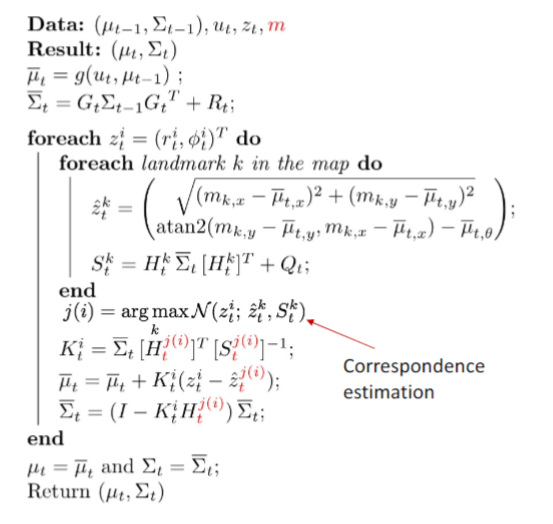
\includegraphics[width=.5\linewidth]{EKFLocatlizationUnknownCoresspondence.png}
\caption{EKF Localization with Unknown Correspondences Algorithm}
\label{fig:UnknownCoresspondences}
\end{figure}

\section{A Taxonomy of Localization problems}
This is a summary of localization problems from Ref. [2] Chapter 7.2 to help us understand the difficulty of a localization problem.

\subsection{Local vs. Global localization}
Local versus global localization can be characterized by the type of knowledge that is available initially
and at run-time.
\begin{enumerate}
    \item \textbf{Position tracking} - the initial robot pose is known. The pose error is small. The uncertainty of Position tracking problem is local problem and confined to region near the robot’s true pose, usually
    \item \textbf{Global localization} - the initial robot pose is unknown. Unimodal probability distributions (e.g., a Gaussian) are usually inappropriate.Thus global localization is more difficult than position tracking.
    \item \textbf{Kidnapped robot problem} - During operation, the robot can get kidnapped and teleported to some other unknown location, thus making localization more difficult. In this case, the robot might believe it knows where it is, while in reality, it does not. Testing a localization algorithm by kidnapping the robot measures its ability to recover from global localization failures.
\end{enumerate}

\subsection{Passive vs. Active Approaches}
Passive versus active approaches distinguishes whether or not the localization algorithm controls the motion of the robot.
\begin{enumerate}
    \item \textbf{Passive localization} - The robot control is independent of the localization process.
    \item \textbf{Active localization} - Active localization algorithms control the robot to minimize the localization error and/or the costs arising from moving a poorly localized robot into a hazardous place.
\end{enumerate}

Active localization algorithm typically perform better than passive ones. But active localization needs to be combined with localization goals and a controlled robot or be built on top of a passive localization algorithm.

\subsection{Single-Robot vs. Multi-Robot}
The difference is the number of robots.
\begin{enumerate}
    \item \textbf{Single-robot localization} - All data is collected at a single robot platform and there is no communication issue.
    \item \textbf{Multi-robot localization} - If all robots work independently, then single-robot localization can be applied for muti-robot localization. The situation becomes complicated when communication happens between them.
\end{enumerate}

\section{Further Reading}
First, we present a few papers that provide extra context and background on the material presented here.
\begin{itemize}
    \item Markov Localization paper: \url{https://www.jair.org/index.php/jair/article/view/10246/24395}
    \item Original Kalman Filter Paper: \url{https://www.cs.unc.edu/~welch/kalman/media/pdf/Kalman1960.pdf}
    \item Estimating the Absolute Position of a Mobile Robot Using Position Probability Grids: \url{http://citeseerx.ist.psu.edu/viewdoc/download?doi=10.1.1.31.7646&rep=rep1&type=pdf}
\end{itemize}

Second, are several articles discussing interesting extensions of this lecture material.

\begin{itemize}
    \item Making use of what you don't see: negative information in Markov localization: \url{https://ieeexplore.ieee.org/abstract/document/1545087}
    \item Markov-Kalman Localization for mobile robots: \url{https://ieeexplore.ieee.org/abstract/document/1048374/references#references}
    \item Episodic non-Markov localization: \url{https://www.sciencedirect.com/science/article/pii/S0921889015302268}
\end{itemize}

\printbibliography

\subsubsection*{Contributors}
Winter 2019: Michael Cai, Nolan Johnson, Hanyuan Liu, Wilson Ruotolo, Allen Zhu, Jiahao Zhang \\
Winter 2018: Arthur Binstein, Anqi Fu, Trevor Halsted, Scott Hemley, Alexander Hobbs, Jialong Wang 

\end{document}